\documentclass[10pt]{amsart}
\usepackage[paperheight=9.55in,paperwidth=6in,margin=0in]{geometry}
%\geometry{landscape}                % Activate for for rotated page geometry
%\usepackage[parfill]{parskip}    % Activate to begin paragraphs with an empty line rather than an indent
\usepackage{graphicx}
\usepackage{amssymb}
\usepackage{epstopdf}
\DeclareGraphicsRule{.tif}{png}{.png}{`convert #1 `dirname #1`/`basename #1 .tif`.png}

% LUKE'S SETTINGS
% packages
\usepackage{framed}
\usepackage{xcolor}
\usepackage{hanging}
% paragraph
\setlength\parindent{0pt}
\setlength{\parskip}{1em}
% margins
%\addtolength{\oddsidemargin}{0.25in}
\addtolength{\topmargin}{0.15in}
%\addtolength{\textheight}{3in}
% frame
\definecolor{shadecolor}{rgb}{0.95,0.95,0.95}
% fixed width font (Courier)
\renewcommand{\ttdefault}{pcr}
% san-serif font (Helvetica)
\usepackage[scaled]{helvet}
\renewcommand\familydefault{\sfdefault} 
\usepackage[T1]{fontenc}
% column widths with any alignment
\usepackage{array}
\newcolumntype{L}[1]{>{\raggedright\let\newline\\\arraybackslash\hspace{0pt}}m{#1}} % left-mid
\newcolumntype{C}[1]{>{\centering\let\newline\\\arraybackslash\hspace{0pt}}m{#1}}   % center-mid
\newcolumntype{R}[1]{>{\raggedleft\let\newline\\\arraybackslash\hspace{0pt}}m{#1}}  % right-mid
\newcolumntype{X}[1]{%
 >{\vbox to 2ex\bgroup\vfill}%
 p{#1}%
 <{\egroup}} 
 
% no extra space after period
\frenchspacing

% Macros file generated by otu_trading_cards.ipynb
\def\sequence{TACGTAGGTGGCAAGCGTTGTCCGGAATTATTGGGCGTAAAGCGCGCGCA
GGCGGTCCTTTAAGTCTGATGTGAAAGCCCACGGCTCAAC}
\def\taxonomyGG{k\_\_Bacteria; p\_\_Firmicutes; c\_\_Bacilli; o\_\_Bacillales; f\_\_Bacillaceae; g\_\_Bacillus; s\_\_foraminis}
\def\taxonomyRDP{d\_\_Bacteria; k\_\_; p\_\_Firmicutes; c\_\_Bacilli; o\_\_Bacillales; f\_\_Bacillaceae 1; g\_\_Bacillus (232/500)}
\def\speciesA{Bacillus sp. (171/500)}
\def\speciesB{Lysinibacillus sp. (51/500)}
\def\speciesC{Planococcus sp. (28/500)}
\def\wikipedia{Did not look up Wikipedia page for Bacillus.}
\def\prevalencePercent{30.70}
\def\prevalenceRank{1}
\def\abundancePercent{0.416}
\def\abundanceRank{16}
\def\numOTUs{155002}
\def\trimLength{90}
\def\numSamples{2000}
\def\rarefactionDepth{5000}


% No page numbers
\thispagestyle{empty}

% Document
\begin{document}

%\begin{framed} % alt: shaded

%\vspace{-6mm}

\begin{center}

\includegraphics[width=12cm]{/Users/luke/Dropbox/UCSD/emp/analyses-otus/emp_logo.pdf}
\end{center}

\hspace{2cm}
\begin{tabular}{L{5in}}
\texttt{\sequence{}}
\end{tabular}

\begin{raggedright}
\begin{hangparas}{2em}{1}
    TAXONOMY:   
    
    \begin{small}
    \begin{tabular}{@{} X{3.5cm} @{ } X{11cm}}
    Greengenes lineage: & \taxonomyGG{} \tabularnewline
    RDP (100\% ID) lineage: & \taxonomyRDP{} \tabularnewline
    RDP (100\% ID) species: & \speciesA{} \speciesB{} \speciesC{} \tabularnewline
    \end{tabular}
	\end{small}

%    WIKIPEDIA:  \wikipedia{}

    PREVALENCE: Found in \prevalencePercent{}\% of samples,
                rank \#\prevalenceRank{} out of \numOTUs{} tag sequences.

    ABUNDANCE:  Composes \abundancePercent{}\% of observations,
                rank \#\abundanceRank{} out of \numOTUs{} tag sequences.
            
    METHODS:    Amplicon PCR with 16S rRNA V4 primers 515f--806rB.
    			Sequencing with Illumina HiSeq 90/100-bp or MiSeq 150-bp single reads.
                Sequences error-checked with Deblur, trimmed to \trimLength{}~bp \& 
                rarefied to \rarefactionDepth{} obs./sample.
                Showing even sample type distribution subset of \numSamples{} samples.

\end{hangparas}

PREVALENCE BY SAMPLE TYPE: \vspace{-7mm}

\begin{tabular}{@{} L{5.5cm} @{ } L{5.4cm} @{} L{4cm}}
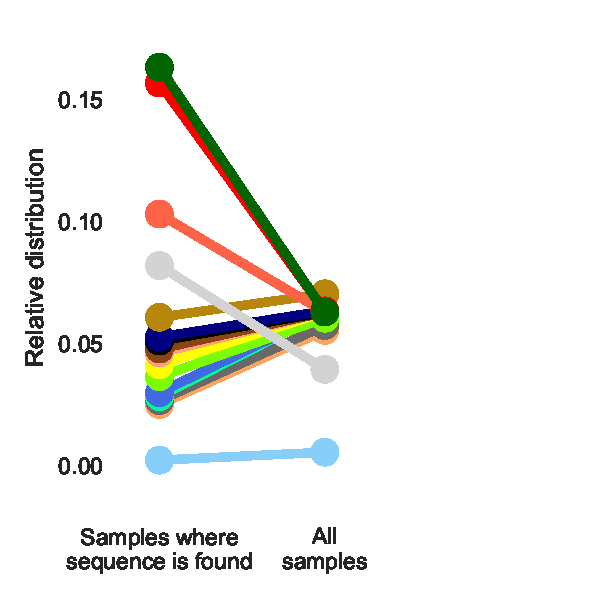
\includegraphics[width=9cm]{point.pdf} & 
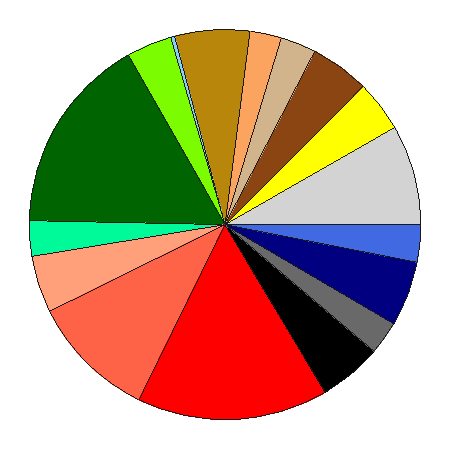
\includegraphics[width=5cm]{pie.pdf} &
\includegraphics[width=4cm]{/Users/luke/Dropbox/UCSD/emp/analyses-otus/empo_legend_portrait.pdf}
\end{tabular}

ABUNDANCE BY ENVIRONMENTAL PARAMETERS:

\vspace{-3mm}

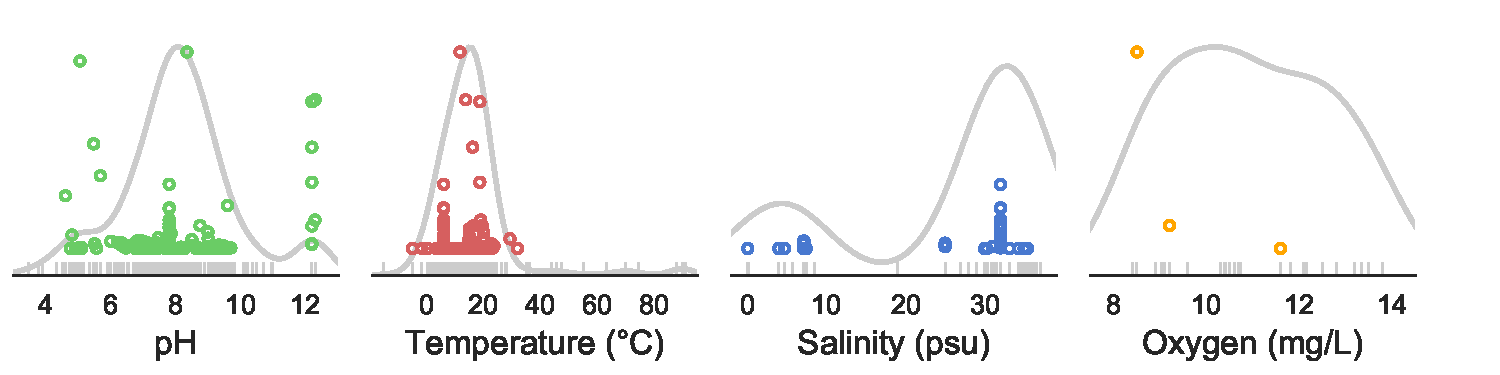
\includegraphics[width=\textwidth]{envparams.pdf}

\end{raggedright}


%\begin{center}
%    \copyright{} 2017 Earth Microbiome Project
%\end{center}

%\end{framed}


\end{document}  